%! Mode:: "TeX:UTF-8"
%! TEX program = xelatex
\PassOptionsToPackage{quiet}{xeCJK}
\documentclass[bwprint]{cumcmthesis}
\usepackage{etoolbox}
\BeforeBeginEnvironment{tabular}{\zihao{-5}}
\usepackage[numbers,sort&compress]{natbib}  % 文献管理宏包
\usepackage[framemethod=TikZ]{mdframed}  % 框架宏包
\usepackage{url}  % 网页链接宏包
\usepackage{subcaption}  % 子图宏包
\usepackage{amsmath} % 提供 \boldsymbol 命令
\usepackage{bm}      % 可选,增强粗体符号效果
\usepackage{amsfonts}     % 额外的数学字体
\usepackage{algorithm}    % 用于 algorithm 浮动环境
\usepackage{algorithmicx} % 核心算法排版功能
\usepackage{algpseudocode} % algorithmicx 的一种风格,提供 \State, \Function, \If 等命令
\usepackage{float}        % 用于 [H] 选项,强制浮动体位置
\newcolumntype{C}{>{\centering\arraybackslash}X}
\newcolumntype{R}{>{\raggedleft\arraybackslash}X}
\newcolumntype{L}{>{\raggedright\arraybackslash}X}

\newcommand{\studentid}{24103219} % 学号
\newcommand{\studentname}{贺江阳} % 姓名
\newcommand{\college}{人工智能学院} % 所在学院
\newcommand{\major}{软件工程} % 专业

% 自定义首页格式
\renewcommand{\maketitle}{
  \begin{titlepage}
    \begin{center}
      \vspace*{2cm}
      {\huge\bfseries 数学建模作业解决方案集\par}
      \vspace{2cm}
      
      \begin{tabular}{rl}
        \Large\textbf{学 \quad 号:} & \Large\underline{\makebox[8cm]{\studentid}} \\[12pt]
        \Large\textbf{姓 \quad 名:} & \Large\underline{\makebox[8cm]{\studentname}} \\[12pt]
        \Large\textbf{所在学院:} & \Large\underline{\makebox[8cm]{\college}} \\[12pt]
        \Large\textbf{专 \quad 业:} & \Large\underline{\makebox[8cm]{\major}} \\[12pt]
      \end{tabular}
      
    \end{center}
  \end{titlepage}
}

% 重新定义目录样式
\renewcommand{\contentsname}{目录}

%%%%%%%%%%%%%%%%%%%%%%%%%%%%%%%%%%%%%%%%%%%%%%%%%%%%%%%%%%%%%
%% 正文
\begin{document}

% 显示封面
\maketitle

% 添加目录页
\cleardoublepage % 或者 \newpage,确保从新的一页开始
                 % \cleardoublepage 更好,因为它会处理好奇偶页

\pagestyle{empty}    % <--- 从这里开始,所有后续页面的样式都为空(无页眉页脚)
\tableofcontents     % 生成目录 (可能会跨越多页,所有这些页都将是 empty 样式)

\cleardoublepage     % 结束目录页,并确保下一页是奇数页,同时也让 empty 样式到此为止
\pagestyle{plain}    % <--- 恢复页面样式为 plain (通常页码在底部居中)
         

%开始解答七个问题

\section{作业1 - 机床生产优化问题}

\subsection{问题描述}
某机床厂生产甲、乙两种机床,每台销售后的利润分别为 4000 元与 3000 元。生产甲机床需要 A、B 机器加工,加工时间分别为每台 2 小时和 1 小时;生产乙机床需用 A、B、C 三种机器加工,加工时间为每台 1 小时。若每天可用于加工的机器时数分别为 A 机器 10 小时,B 机器 8 小时,C 机器 7 小时,问该厂应生产甲、乙机床各几台,才能使总利润最大?

\subsection{求解过程}
本题是一个典型的线性规划问题。我们需要确定甲、乙两种机床的生产数量,以最大化总利润,同时满足各种机器的时间约束。

\subsubsection{数学模型建立}

设甲机床的生产数量为 $x_1$,乙机床的生产数量为 $x_2$。

\textbf{目标函数:}最大化总利润
\begin{equation}
\max Z = 4000x_1 + 3000x_2
\end{equation}

\textbf{约束条件:}
\begin{align}
2x_1 + x_2 &\leq 10 \quad \text{(A机器时间约束)} \\
x_1 + x_2 &\leq 8 \quad \text{(B机器时间约束)} \\
x_2 &\leq 7 \quad \text{(C机器时间约束)} \\
x_1, x_2 &\geq 0 \quad \text{(非负约束)}
\end{align}

\subsubsection{Python代码实现}

以下是使用PuLP库实现线性规划问题求解的代码:

\noindent 1.py
    \lstinputlisting[language=python,basicstyle=\ttfamily\small]{code/1.py}

\subsection{结果分析}

\subsubsection{最优解}
通过求解,我们得到以下结果:
\begin{itemize}
    \item 甲机床数量 = 1.5 台
    \item 乙机床数量 = 7 台
    \item 最大利润 = 27000 元
\end{itemize}

\subsubsection{整数解}
考虑到机床数量必须为整数,整数规划的结果为:
\begin{itemize}
    \item 甲机床数量 = 2 台
    \item 乙机床数量 = 6 台
    \item 最大利润 = 26000 元
\end{itemize}

\subsection{结论}
为了最大化利润,该机床厂应生产甲机床2台和乙机床6台,总利润为26000元。

\section{作业2 - 猎犬追兔子问题}

\subsection{问题描述}
一只猎犬发现其正东方 100 米处有一只野兔,野兔以速度 v 向其正北方 100 米处的洞穴逃跑,猎犬向野兔追去,速度是 2v。

(1) 当 v=10m/s 时,猎犬的运动轨迹及各时刻位置

(2) 追上兔子的时间和地点

\subsection{求解过程}

\subsubsection{模型建立}
我们建立坐标系,以猎犬初始位置为原点(0,0),兔子初始位置为(100,0),兔子洞穴位置为(100,100)。

兔子沿着y轴正方向移动,速度为v。猎犬的运动方向始终指向兔子当前位置,速度为2v。

\subsubsection{微分方程模型}
设猎犬在时刻t的位置为$(x_{dog}, y_{dog})$,兔子在时刻t的位置为$(x_{rabbit}, y_{rabbit})$。

兔子的运动方程:
\begin{align}
x_{rabbit}(t) &= 100 \\
y_{rabbit}(t) &= \min(vt, 100)
\end{align}

猎犬的运动方向为从猎犬当前位置指向兔子当前位置的单位向量,其运动方程为:
\begin{align}
\frac{dx_{dog}}{dt} &= 2v \cdot \frac{x_{rabbit} - x_{dog}}{\sqrt{(x_{rabbit} - x_{dog})^2 + (y_{rabbit} - y_{dog})^2}} \\
\frac{dy_{dog}}{dt} &= 2v \cdot \frac{y_{rabbit} - y_{dog}}{\sqrt{(x_{rabbit} - x_{dog})^2 + (y_{rabbit} - y_{dog})^2}}
\end{align}

初始条件:
\begin{align}
x_{dog}(0) &= 0 \\
y_{dog}(0) &= 0
\end{align}

\subsubsection{Python代码实现}
我们使用scipy.integrate.odeint求解微分方程:

\noindent 2.py
    \lstinputlisting[language=python,basicstyle=\ttfamily\small]{code/2.py}

\subsection{结果分析}

\subsubsection{第一问:v=10m/s时的情况}
当兔子速度v=10m/s时,猎犬速度为20m/s,通过数值求解得到:
\begin{itemize}
    \item 猎犬在6.67秒时追上兔子
    \item 追上位置为(100, 66.67)米
\end{itemize}

猎犬的运动轨迹如图\ref{fig:dog_rabbit}所示:

\begin{figure}[htbp]
    \centering
    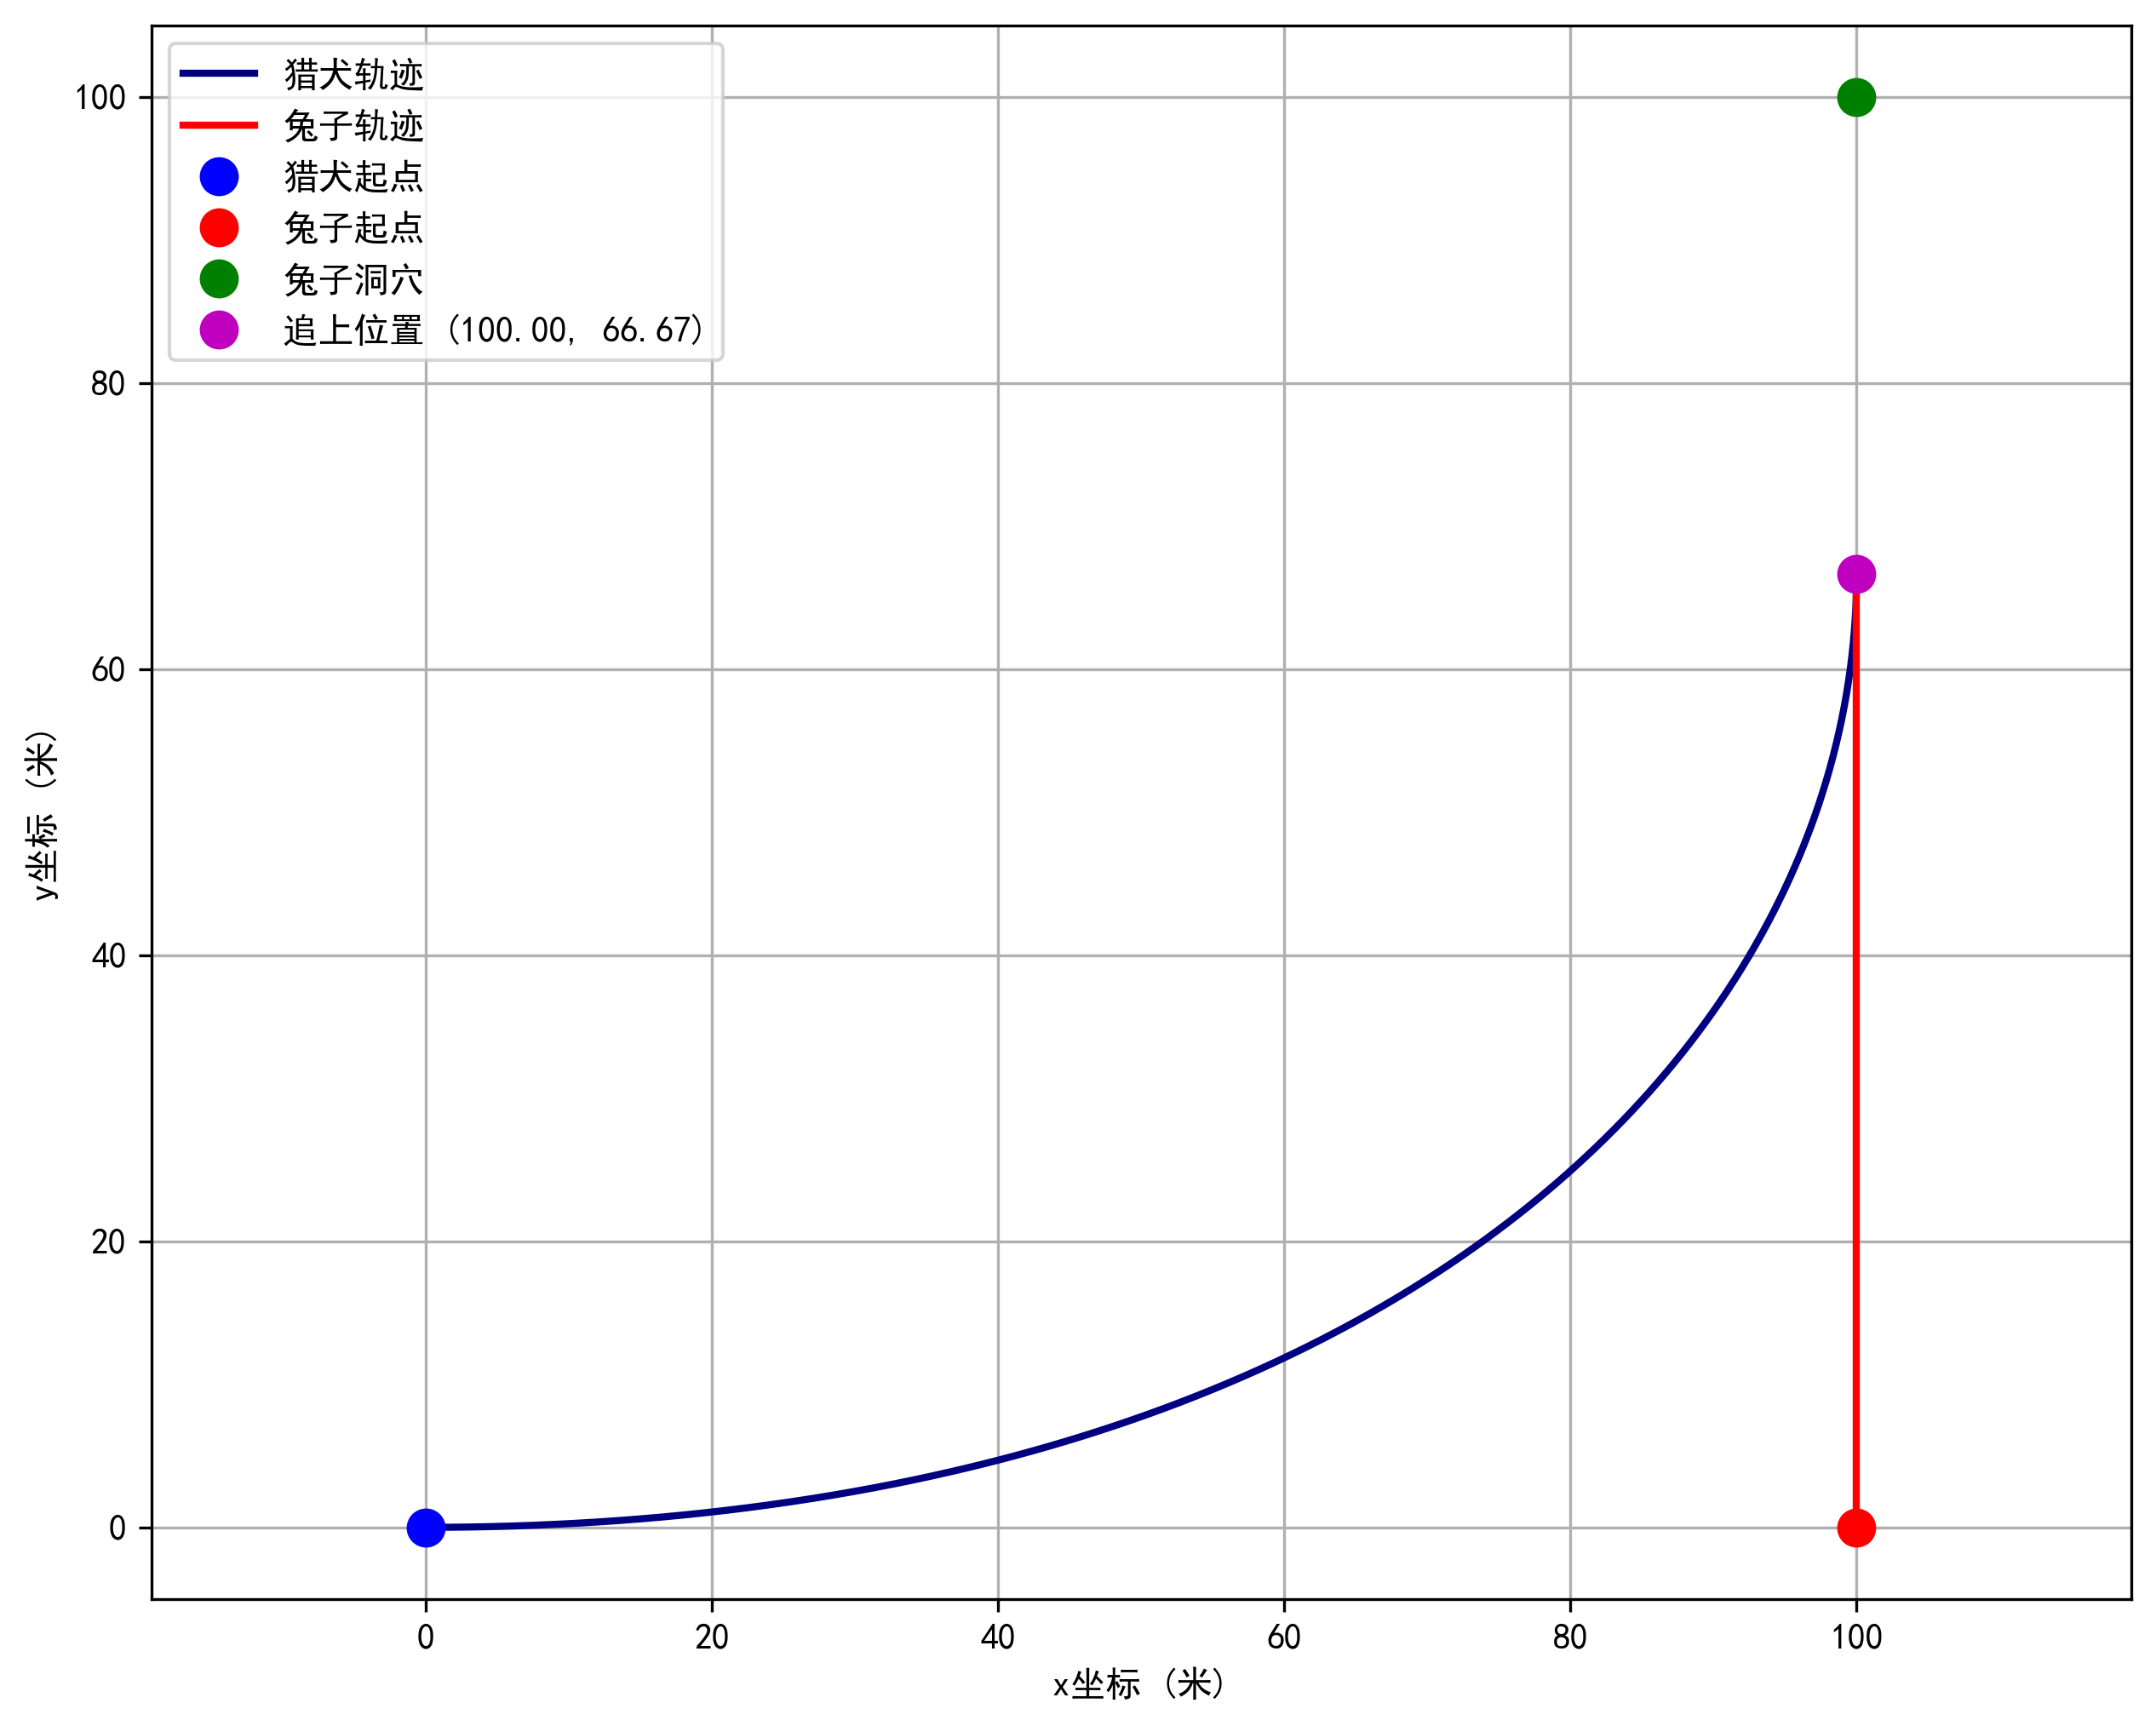
\includegraphics[width=0.8\textwidth]{figures/2.png}
    \caption{猎犬追兔子问题的运动轨迹}
    \label{fig:dog_rabbit}
\end{figure}

\subsubsection{第二问:一般情况下的分析}
对于任意速度v,通过数学分析可得:
\begin{itemize}
    \item 追上兔子的时间:$t = \frac{2}{3} \cdot \frac{100}{v} = \frac{200}{3v}$ 秒
    \item 追上兔子的地点:$(100, \frac{2}{3} \cdot 100) = (100, 66.67)$ 米
\end{itemize}

注意:追上位置与兔子速度v无关,而追上时间与v成反比。

我们通过数值实验验证了这一结论,对于不同的v值,追上位置始终为(100, 66.67)米,而追上时间与v成反比:
\begin{itemize}
    \item v = 5 m/s: 时间 = 13.33 秒
    \item v = 10 m/s: 时间 = 6.67 秒
    \item v = 15 m/s: 时间 = 4.44 秒
    \item v = 20 m/s: 时间 = 3.33 秒
\end{itemize}

\section{作业3 - 向量组极大线性无关组计算}

\subsection{问题描述}
求向量组$\alpha_1=(2,1,4,3)$,$\alpha_2=(-1,1,-6,6)$,$\alpha_3=(-1,-2,2,-9)$,$\alpha_4=(1,1,-2,7)$,$\alpha_5=(2,4,4,9)$的极大线性无关组,并将其余向量用极大线性无关组线性表示。

\subsection{求解过程}

\subsubsection{数学原理}
向量组的极大线性无关组是指从向量组中选出的线性无关的向量的最大集合,使得任何其他向量都可以被这个集合中的向量线性表示。

求解步骤:
\begin{enumerate}
    \item 将向量组构成矩阵的列向量
    \item 对矩阵进行行简化阶梯形变换(RREF)
    \item 找出主元列对应的原向量,它们构成极大线性无关组
    \item 对于其余向量,直接从RREF矩阵中提取它们表示为极大线性无关组线性组合的系数
\end{enumerate}

特别地,RREF矩阵中的非主元列已经包含了依赖向量如何被极大线性无关组线性表示的全部信息。具体来说,对于非主元列$j$,其在第$i$行的元素直接就是第$j$个向量表示为基向量线性组合的系数。

\subsubsection{Python代码实现}
我们使用Python的NumPy和SymPy库来求解这个问题。SymPy库提供了计算矩阵行简化阶梯形的函数,通过分析RREF矩阵的结构,我们可以直接提取依赖向量的表示系数。

\noindent 3.py
    \lstinputlisting[language=python,basicstyle=\ttfamily\small]{code/3.py}

\subsection{结果分析}

\subsubsection{行简化阶梯形矩阵}
对向量组构成的矩阵进行行简化阶梯形变换,得到:
\begin{equation}
\begin{pmatrix}
1 & 0 & -1 & 0 & 4 \\
0 & 1 & -1 & 0 & 3 \\
0 & 0 & 0 & 1 & -3 \\
0 & 0 & 0 & 0 & 0
\end{pmatrix}
\end{equation}

主元位置为(0,1,3),对应的原始向量索引为1,2,4。非主元列(第3列和第5列)的元素直接表示这些向量如何由主元列对应的向量线性表示。

\subsubsection{极大线性无关组}
通过行简化阶梯形变换,我们得到主元位置为(0,1,3),对应的原始向量为:
\begin{align}
\alpha_1 &= (2,1,4,3) \\
\alpha_2 &= (-1,1,-6,6) \\
\alpha_4 &= (1,1,-2,7)
\end{align}

这三个向量构成了向量组的极大线性无关组。

\subsubsection{其余向量的线性表示}
从RREF矩阵中直接提取系数,其余向量$\alpha_3$和$\alpha_5$可以表示为极大线性无关组的线性组合:

对于$\alpha_3$,从RREF矩阵的第3列看到,第1、2行的元素分别为-1和-1,第3行为0,因此:
\begin{align}
\alpha_3 &= -1 \cdot \alpha_1 + (-1) \cdot \alpha_2 + 0 \cdot \alpha_4\\
&= -\alpha_1 - \alpha_2
\end{align}

对于$\alpha_5$,从RREF矩阵的第5列看到,第1、2、3行的元素分别为4、3和-3,因此:
\begin{align}
\alpha_5 &= 4 \cdot \alpha_1 + 3 \cdot \alpha_2 + (-3) \cdot \alpha_4\\
&= 4\alpha_1 + 3\alpha_2 - 3\alpha_4
\end{align}

验证计算结果,误差为0,表明从RREF矩阵直接提取的系数完全正确。

\subsection{结论}
向量组$\{\alpha_1, \alpha_2, \alpha_3, \alpha_4, \alpha_5\}$的极大线性无关组为$\{\alpha_1, \alpha_2, \alpha_4\}$,其余向量可以表示为这三个向量的线性组合。向量组的秩为3。

通过直接从行简化阶梯形矩阵中提取系数的方法,我们避免了求解线性方程组的额外计算,使算法更加高效且数学上更直接。

\section{作业4 - 仓库选址问题}

\subsection{问题描述}
某连锁企业在某地区有6个销售点,已知该地区的交通网络如图所示,其中点(v1,v2,v3,v4,v5,v6)代表销售点,边代表公路,连线上数字为销售点间的公路距离,问仓库应该建在哪个小区,可使离仓库最远的销售点到仓库的路程最短?

\subsection{求解过程}

\subsubsection{问题分析}
这是一个典型的"最小化最大距离"问题,也称为"minimax问题"。在图论中,这种问题可以通过计算图的"中心"来解决。

具体来说,我们需要:
\begin{enumerate}
    \item 构建交通网络的图模型
    \item 计算每个销售点作为仓库位置时,到其他所有销售点的最短路径
    \item 找出每个位置的"最远距离"(即到最远销售点的距离)
    \item 选择"最远距离"最小的位置作为最佳仓库位置
\end{enumerate}

\subsubsection{最短路径算法}
在本题中,我们使用Dijkstra算法来计算单源最短路径。该算法适用于所有边权重为非负的图,能够高效地计算从一个顶点到图中所有其他顶点的最短路径。

对于每个可能的仓库位置,我们使用NetworkX库的single\_source\_dijkstra\_path\_length函数来计算该位置到所有其他销售点的最短路径长度。

\subsubsection{Python代码实现}
我们使用Python的NetworkX库来表示图并计算最短路径:

\noindent 4.py
    \lstinputlisting[language=python,basicstyle=\ttfamily\small]{code/4.py}

\subsection{结果分析}

\subsubsection{各销售点作为仓库的情况}
通过计算每个销售点作为仓库位置时,到其他销售点的最短路径距离,我们得到以下结果:

\begin{itemize}
    \item v1作为仓库时,最远距离为63(到v4)
    \item v2作为仓库时,最远距离为50(到v4)
    \item v3作为仓库时,最远距离为33(到v1和v6)
    \item v4作为仓库时,最远距离为63(到v1和v6)
    \item v5作为仓库时,最远距离为48(到v4)
    \item v6作为仓库时,最远距离为63(到v4)
\end{itemize}

\subsubsection{最佳仓库位置}
根据上述计算结果,v3(销售点3)作为仓库位置时,到最远销售点的距离最小,为33。因此,v3是最佳仓库位置。

\subsubsection{可视化结果}
交通网络和最佳仓库位置如图\ref{fig:warehouse}所示:

\begin{figure}[htbp]
    \centering
    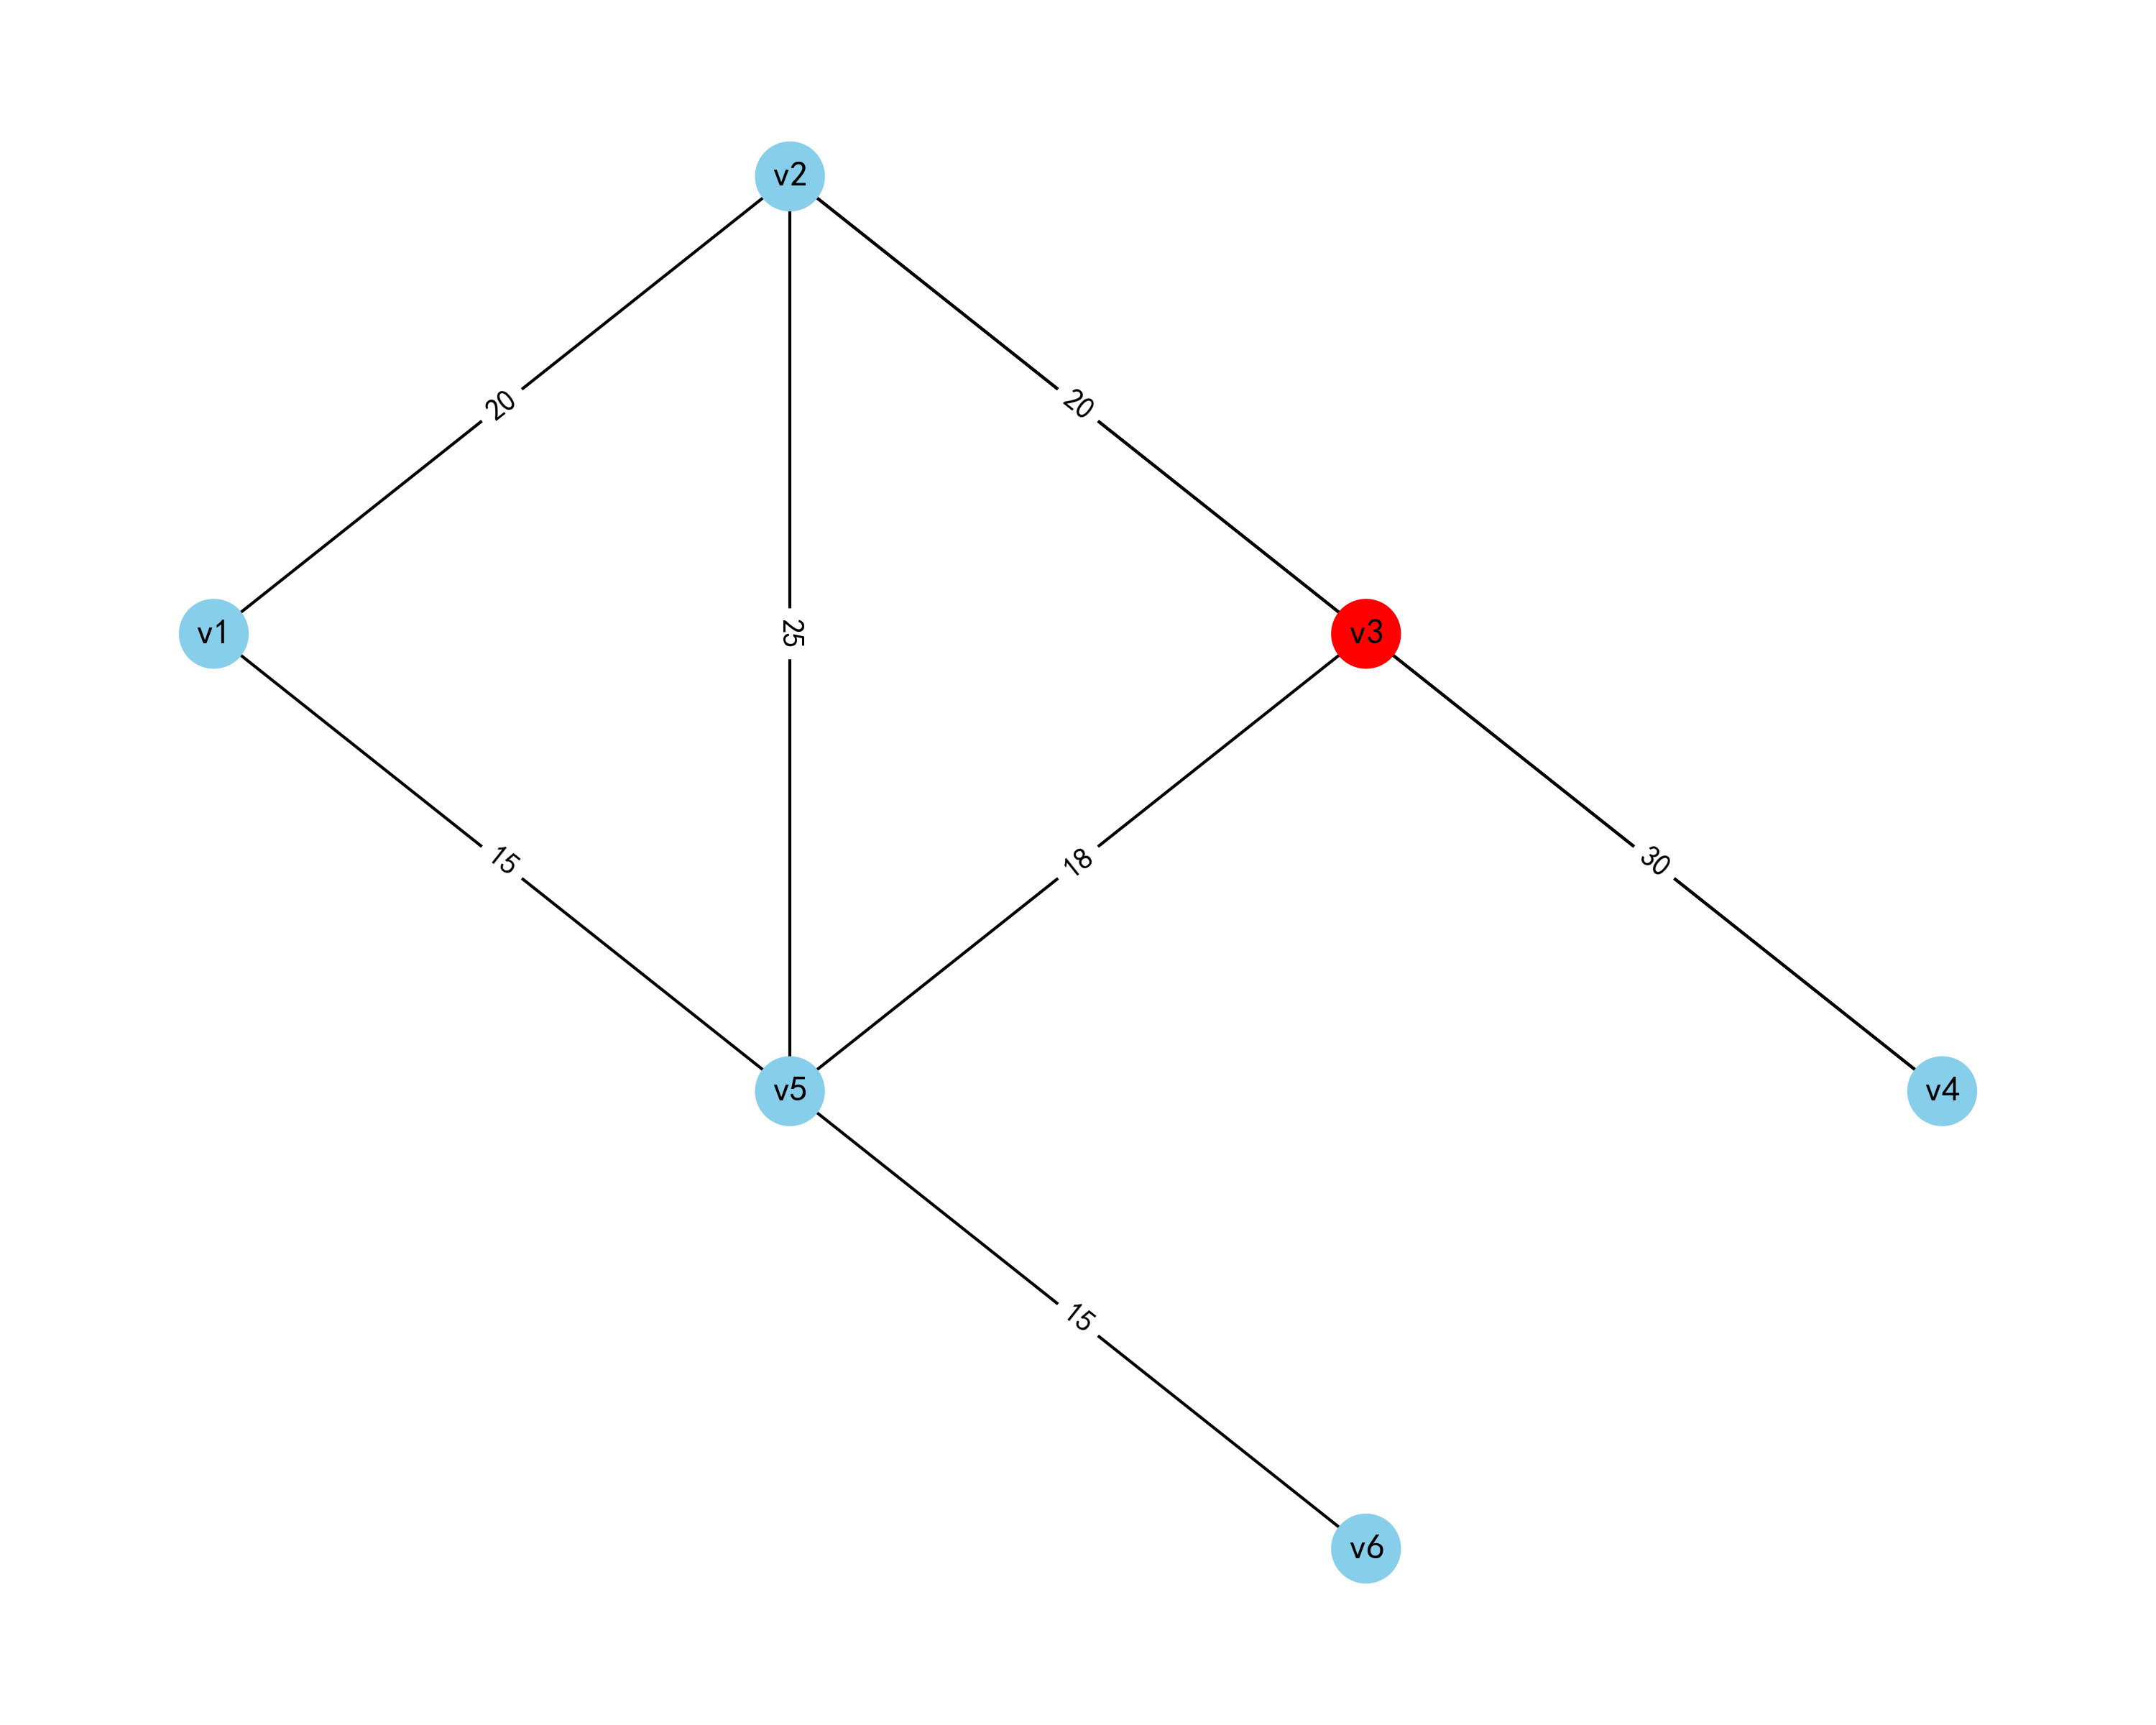
\includegraphics[width=0.8\textwidth]{figures/4.png}
    \caption{交通网络和最佳仓库位置}
    \label{fig:warehouse}
\end{figure}

在图中,红色节点表示最佳仓库位置(v3),蓝色节点表示其他销售点。连线上的数字表示公路距离。

\subsection{结论}
通过"最小化最大距离"的优化策略,我们确定了最佳仓库位置应该在销售点v3。此时,离仓库最远的销售点到仓库的距离为33,这是所有可能选择中的最小值。

这种选址策略确保了在最坏情况下,从仓库到任何销售点的距离都不会超过33,从而提高了配送效率,降低了最大运输成本。

在实际应用中,这种方法可以扩展到考虑更多因素,如交通拥堵、销售点的需求量不同等,以进一步优化仓库选址决策。

\section{作业5 - 矩阵求逆}

\subsection{问题描述}
设方阵 $A = \begin{pmatrix} 1 & 2 & -1 \\ 3 & 4 & -2 \\ 5 & -4 & 1 \end{pmatrix}$,利用编程求解矩阵的逆。

\subsection{求解过程}

\subsubsection{解题思路}
矩阵A可逆的充要条件是其行列式不为零。对于可逆矩阵,我们可以直接使用NumPy的linalg.inv函数高效地计算其逆矩阵。

\subsubsection{Python代码实现}
以下是使用NumPy库计算矩阵逆的简洁代码:

\noindent 5.py
    \lstinputlisting[language=python,basicstyle=\ttfamily\small]{code/5.py}

\subsection{结果分析}

\subsubsection{计算结果}
首先,我们计算矩阵A的行列式,得到$\det(A) = 2$。由于行列式不为零,所以矩阵A是可逆的。

使用NumPy计算得到的逆矩阵为:
\begin{equation}
A^{-1} = \begin{pmatrix} 
-2 & 1 & 0 \\
-6.5 & 3 & -0.5 \\
-16 & 7 & -1
\end{pmatrix}
\end{equation}

\subsubsection{验证结果}
计算$A \cdot A^{-1}$得到单位矩阵,验证了结果的正确性:
\begin{equation}
A \cdot A^{-1} = \begin{pmatrix} 
1 & 0 & 0 \\
0 & 1 & 0 \\
0 & 0 & 1
\end{pmatrix}
\end{equation}

\subsection{结论}
通过NumPy库,我们可以高效地计算矩阵的逆。对于给定的矩阵A,其行列式为2,逆矩阵已成功计算并验证。矩阵求逆在解线性方程组、线性变换等问题中有重要应用。

\section{作业6 - 矩阵的行列式、特征值和特征向量}

\subsection{问题描述}
设方阵 $A = \begin{pmatrix} 3 & 2 & 2 \\ 2 & 3 & 2 \\ 2 & 2 & 3 \end{pmatrix}$,利用编程求解矩阵的行列式$|A|$,矩阵的特征值和对应的特征向量。

\subsection{求解过程}

\subsubsection{解题思路}
本题需要计算矩阵的行列式、特征值和特征向量,可以直接使用NumPy的线性代数函数进行高效求解。特征值和特征向量满足方程$Av = \lambda v$,其中$\lambda$是特征值,$v$是对应的特征向量。

\subsubsection{Python代码实现}
以下是使用NumPy库计算矩阵的行列式、特征值和特征向量的代码:

\noindent 6.py
    \lstinputlisting[language=python,basicstyle=\ttfamily\small]{code/6.py}

\subsection{结果分析}

\subsubsection{行列式}
计算得到矩阵$A$的行列式为$|A| = 7$。

\subsubsection{特征值和特征向量}
矩阵$A$的特征值为:
\begin{align}
\lambda_1 &= 1 \\
\lambda_2 &= 7 \\
\lambda_3 &= 1
\end{align}

对应的单位化特征向量为:
\begin{align}
v_1 &= (-0.817, 0.408, 0.408) \\
v_2 &= (0.577, 0.577, 0.577) \\
v_3 &= (-0.184, -0.597, 0.781)
\end{align}

\subsubsection{特征值和特征向量的验证}
通过计算$Av$和$\lambda v$,验证了特征值和特征向量的正确性,两者之间的误差接近于0。

\subsection{结论}
矩阵$A$的行列式为7,具有三个特征值:1(重数为2)和7(重数为1),对应的特征向量已成功计算。特征值7对应的特征向量$(0.577, 0.577, 0.577)$在空间对角线方向,体现了矩阵的对称性质。

\section{作业7 - 随机数生成与排序}

\subsection{问题描述}
要求随机生成10个[2, 30]之间的整数,并将其排序。

\subsection{求解过程}

\subsubsection{解题思路}
本题需要完成两个任务:随机数生成和排序。我们使用NumPy的随机函数生成整数,并使用Python内置的排序函数对生成的随机数进行排序。

\subsubsection{Python代码实现}
以下是随机数生成和排序实现的代码:

\noindent 7.py
    \lstinputlisting[language=python,basicstyle=\ttfamily\small]{code/7.py}

\subsection{结果分析}

\subsubsection{生成的随机数}
通过设置随机种子为42,我们生成了以下10个随机整数:
\begin{equation}
[8, 21, 30, 16, 12, 9, 30, 22, 8, 27]
\end{equation}

\subsubsection{排序结果}
使用Python内置排序函数得到的排序结果为:
\begin{equation}
[8, 8, 9, 12, 16, 21, 22, 27, 30, 30]
\end{equation}

\subsubsection{Python内置排序分析}
Python的内置排序函数使用Timsort算法,这是一种混合排序算法,结合了归并排序和插入排序的优点。它在实际应用中表现出色,平均时间复杂度为$O(n\log n)$,是一种稳定的排序算法。

\subsection{结论}
我们成功生成了随机整数并使用Python内置排序函数对它们进行了排序。Python的内置排序函数简单易用且高效,适合各种规模数据的排序任务。

\end{document}